%
% teil2.tex -- Beispiel-File für teil2 
%
% (c) 2020 Prof Dr Andreas Müller, Hochschule Rapperswil
%
% !TEX root = ../../buch.tex
% !TEX encoding = UTF-8
%
\section{Herleitung der Balkengleichung
	\label{balken:section:teil2}}
\subsection{Variationsprinzip}
Die Variationsrechnung ist ein Teilgebiet der Analysis, das sich mit kleinen Änderungen in Funktionen und Funktionalen beschäftigt, um Minima und Maxima von Funktionen zu ermitteln. Dabei handelt es sich um mathematische Ausdrücke, die Integrale über eine unbekannte Funktion und ihre Ableitung darstellen können. Ziel ist es, ein Maximum, ein Minimum oder einen Sattelpunkt ausfindig zu machen.

In der Mechanik kommen Variationsrechnungen oft zum Einsatz, da sie die Grundlage aller physikalischen Extremalrechnungen bilden \cite{balken:Variationsrechnung}.

\subsection{Minimalprinzip}
Das Minimalprinzip ist ein Konzept, das besagt, dass ein physikalisches System einen Zustand annimmt, der mit dem geringsten Energieaufwand erreicht wird. In der Physik wird das Minimalprinzip oft formuliert, indem eine minimale Wirkung oder Energie angestrebt wird.

Ein Beispiel hierfür ist eine Feder, die an einem Ende an einer Wand befestigt ist und an ihrem anderen Ende eine Masse trägt. Zieht man die Masse nach unten und lässt sie los, nimmt sie eine Position ein, bei der die potenzielle Energie minimal ist.

Das Minimalprinzip in Bezug auf die Balkengleichung ist ein grundlegendes Konzept der Mechanik, auch bekannt als das Prinzip von Hamilton. Es besagt, dass ein System den Gleichgewichtszustand annimmt, bei dem die potenzielle Energie minimal ist. Für einen Balken tritt dieser Zustand ein, wenn alle äusseren Kräfte, Momente, inneren Beanspruchungen sowie Verformungen des Balkens im Gleichgewicht stehen. Die Anwendung dieses Minimalprinzips führt zur Balkengleichung, die die Gleichgewichtsbedingungen des Balkens beschreibt. 

\subsection{Herleitung der Balkengleichung aus dem Variationsprinzip}
Die Verformungen des Balkens aufgrund der auftretenden Biegespannungen $\sigma_x$ werden durch
\begin{equation}
	\sigma_x = \frac{E}{\varrho} z
\end{equation}
und
\begin{equation}
	\sigma_x = \frac{M_y}{I_y} z
\end{equation}
beschrieben. Setzt man diese beiden Gleichungen gleich, erhält man
\begin{equation}
	\frac{E}{\varrho} z = \frac{M_y}{I_y} z
\end{equation}
und kürzt anschliessend $z$ heraus, so bekommt man
\begin{equation}
	\frac{E}{\varrho} = \frac{M_y}{I_y}.
\end{equation}
Dividiert man diese Gleichung durch $E$, um $\varrho$ zu isolieren, erhält man die Formel für den Krümmungsradius
\begin{equation}
	\frac{1}{\varrho} = \frac{M_y}{E I_y} = \kappa.
\end{equation}

Bei Biegungen, die aufgrund von Querkräften auftreten, ist das Moment veränderlich und hängt von der Position $x$ ab. Dies führt dazu, dass die Krümmung des Balkens bzw. der Biegelinie von der Position $x$ abhängt. Um die Krümmung zu bestimmen, benötigt man den kürzesten Weg zwischen beiden Auflagern des Balkens.
\begin{figure}
	\centering
	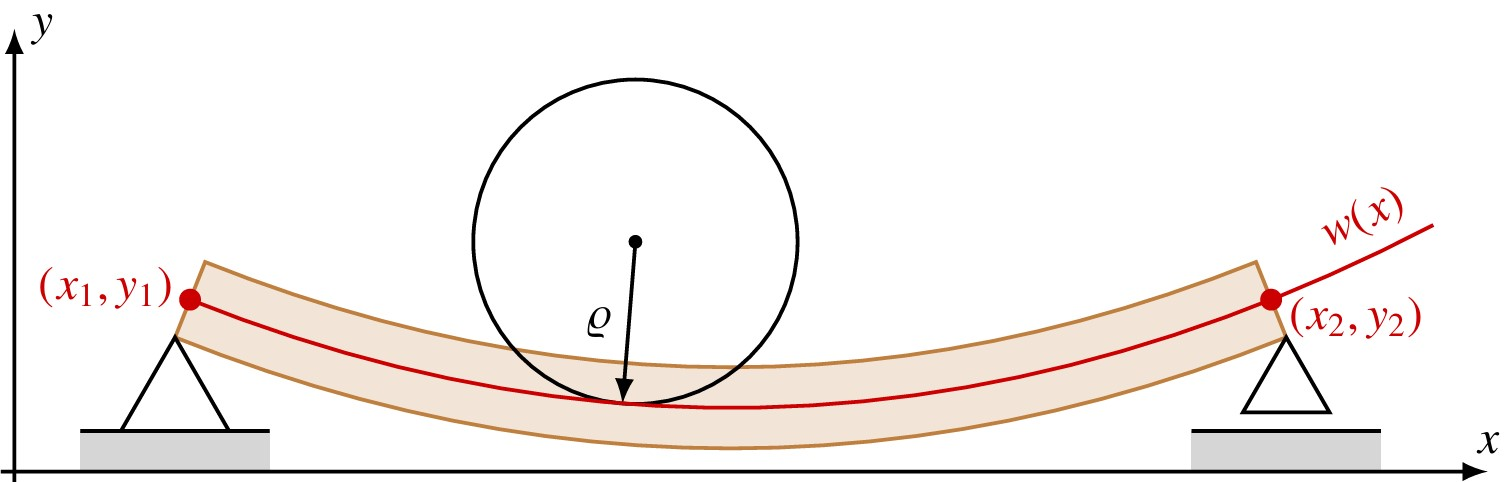
\includegraphics[width=0.8\textwidth]{papers/balken/images/teil2/BiegungBalke2.jpg}
	\caption{Darstellung der Biegelinie $y(x)$ mit dem Balken (rot gekennzeichnet) und dessen Auflagern.}
	\label{fig:Darstellung_der_Biegelinie}
\end{figure}

Zuerst berechnet man die Länge einer Geraden auf der Kurve $y(x)$:
\begin{equation}
	\Delta s = \sqrt{\Delta x^2 + \Delta y^2} \approx \sqrt{1 + y'(x)^2} \cdot \Delta x
\end{equation}
und danach mit dem Integral die Kurvenlänge $l(y)$:
\begin{equation}
	l(y) = \int_{x_1}^{x_2} \sqrt{1 + {y'(x)}^2} \, dx.
\end{equation}

\subsection{Variationsprinzip für die potentielle Energie}
Um das Variationsprinzip auf die Balkengleichung anwenden zu können, betrachtet man die potenzielle Energie des Balkens. Diese setzt sich aus der Biegeenergie sowie der Energie der äusseren Kräfte zusammen. Die potenzielle Energie im Balken wird minimiert, wenn sich das System im Gleichgewicht befindet.
\begin{figure}
	\centering
	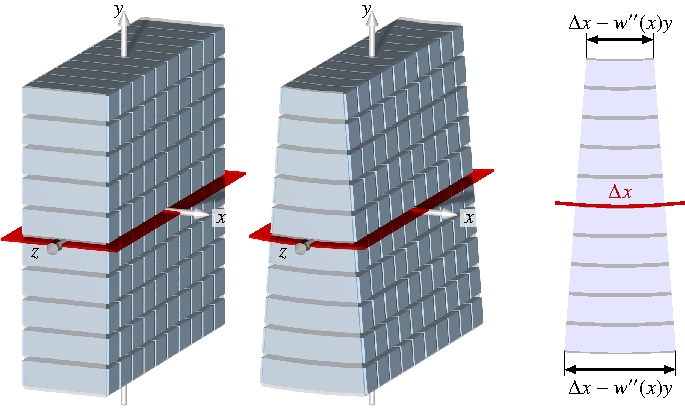
\includegraphics[width=0.8\textwidth]{papers/balken/images/teil2/federgesetz.pdf}
	\caption{Veranschaulichung zur Energie im Balken durch das Flächenträgheitsmoment}
	\label{fig:Veranschaulichung zur Energie im Balken durch das Flächenträgheitsmoment}
\end{figure}

Die Energiedichte des Balkens an einem Punkt $x$ ist gegeben durch
\begin{equation}
	\frac{1}{2} E I \left( \frac{\partial^2 w}{\partial x^2} \right)^2.
\end{equation}
Hierbei ist $E I$ das Produkt aus dem Elastizitätsmodul und dem Flächenträgheitsmoment $I$, $w(x)$ beschreibt die Durchbiegung des Balkens.

Zusätzlich zur inneren Energie kommt noch die Last $q(x)$, sodass das Funktional der Euler-Bernoulli-Gleichung wie folgt aussieht:
\begin{equation}
	\int_0^L \left( -\frac{1}{2} \left( \frac{\partial^2 w}{\partial x^2} \right)^2 + q(x) w(x) \right) \, dx.
\end{equation}

\subsection{Zeitabhängige Durchbiegung}
Für zeitabhängige Durchbiegungen $w(x,t)$ kommt noch ein kinetischer Energieterm hinzu:
\begin{equation}
	\frac{1}{2} \mu \left( \frac{\partial w}{\partial t} \right)^2.
\end{equation}

\subsection{Differentialgleichung für $w(x)$}
Die Lagrange-Funktion lautet daher:
\begin{equation}
	L(x,w,w',w'') = -\frac{1}{2} E I (w'')^2 + q w.
\end{equation}
Die Ableitungen der Lagrange-Funktion ergeben:
\begin{align}
	\frac{\partial L}{\partial w} &= q \\
	\frac{\partial L}{\partial w'} &= 0 \\
	\frac{\partial L}{\partial w''} &= -E I w''.
\end{align}
Da die Lagrange-Funktion eine höhere Ableitung enthält, erweitert sich die Euler-Lagrange-Differentialgleichung zu:
\begin{equation}
	\frac{\partial L}{\partial w} - \frac{d}{dx} \frac{\partial L}{\partial w'} + \frac{d^2}{dx^2} \frac{\partial L}{\partial w''} = 0.
\end{equation}
Einsetzen der Ableitungen ergibt:
	\begin{align}
		q - \frac{d^2}{dx^2}(E I w'') &= 0 \\
		\Rightarrow w''''(x) &= \frac{q}{E I}.
	\end{align}

\subsection{Krümmung}
Unsere Lagrange-Funktion ist somit:
\begin{equation}
	L(x,y,y') = \sqrt{1 + {y'}^2}
\end{equation}
Die partiellen Ableitung von $L$ sind:
\begin{equation}
	\frac{\partial L}{\partial y} = 0
\end{equation}
und
\begin{equation}
	\frac{\partial L}{\partial y'} = \frac{y'}{\sqrt{1 + {y'}^2}}.
\end{equation}

Setzt man $y(x)$ ein und leitet nach $x$ ab, ergibt sich:
\begin{equation}
	\frac{d}{dx} \frac{\partial L}{\partial y'}(x,y(x),y'(x)) = \frac{d}{dx} \frac{y'(x)}{\sqrt{1 + {y'}^2}} = \frac{(1 + {y'(x)}^2 - {y'(x)}^2) y''(x)}{(1 + {y'(x)}^2)^{\frac{3}{2}}}.
\end{equation}
Dies führt zu:
\begin{equation}
	\frac{d}{dx} \frac{\partial L}{\partial y'}(x,y(x),y'(x)) = \frac{y''}{(1 + {y'}^2)^{\frac{3}{2}}}.
\end{equation}

Die rechte Seite davon ist die Krümmung
\begin{equation}
	\kappa = \frac{1}{\varrho} = \pm \frac{y''}{(1 + {y'}^2)^{\frac{3}{2}}}.
\end{equation}

Da wir in unserem Fall $w(x)$ als Funktion für die Biegelinie verwenden, müssen wir das Vorzeichen bestimmen. Da ein positives Moment eine Biegung nach unten verursacht, müssen wir ein negatives Vorzeichen verwenden. Somit erhalten wir:
\begin{equation}
	\kappa=
	\frac{1}{\varrho}=
	-\frac{w''}{\left(1+{w'}^2\right)^\frac{3}{2}}
\end{equation}
mit
\begin{equation}
	w'=
	\frac{dy}{dx} 
\end{equation}
und
\begin{equation}
	w''=
	\frac{d^2y}{dx^2}
\end{equation}

$w$ = Funktion der Durchbiegung

$w'$ = Neigung der Durchbiegung

$w''$ = Krümmung

Da wir in der Baustatik den Rechtssystem verwenden, kehren wir die $z$-Achse so, dass nach unten das positive Vorzeichen ist (siehe Abbildung 13.9).
\begin{figure}
\centering
	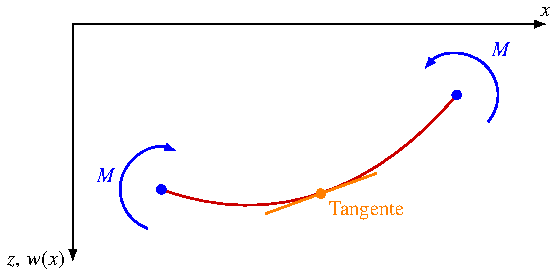
\includegraphics[width=0.8\textwidth]{papers/balken/images/teil2/BiegungverdrehteAchsen.pdf}
\caption{Abbildung von den verdrehten $z$-Achse und die positive Momenten, welche auf der Biegelinie wirken.}
\label{fig:Abbildung von den verdrehten $z$-Achse und die positive Momenten, welche auf der Biegelinie wirken.}
\end{figure}

Unsere Funktion zeigt eine Krümmung nach links, jedoch durch die Spiegelung an der $z$-Achse ergibt sich eine Krümmung nach rechts.
Bei Rechtskrümmungen sind die 2. Ableitungen kleiner als 0: $w'' < 0$.
Das ergibt
\begin{equation}
	\kappa=
	-\frac{w''}{\left(1+{w'}^2\right)^\frac{3}{2}}=
	\frac{M_y}{EI_y}.
\end{equation}
Der Term $w’$ kann vernachlässigt werden, da im Betracht des Hookesche Gesetz nur kleine Verformungen vorliegen.
Daraus ergeben sich Tangentensteigungen von $w’ << 1$.
\begin{equation}
	\kappa=
	-\frac{w''}{\left(1+{w'}^2\right)^\frac{3}{2}}=
	-\frac{w''}{\left(1+0\right)^\frac{3}{2}}=
	-\frac{w''}{1}=-w''=
	\frac{M_y}{EI_y}.
\end{equation}
Daraus ergibt sich:
\begin{equation}
	w''=
	-\frac{M_y}{EI_y}
\end{equation}
mit
\begin{equation}
	\kappa=
	-w''.
\end{equation}

\subsection{Temperatureinflüsse}
Temperaturunterschiede verursachen Verformungen in der Balkenachse.
Daher ist es wichtig, die Krümmung der Biegelinie bei Temperaturänderungen zu berücksichtigen.
Daraus ergibt sich der Formel.
\begin{equation}
	w''=
	-\frac{M_y}{EI_y}-\alpha_{\text{th}}\frac{\Delta T}{h}
\end{equation}

$α_th$ = thermische Ausdehnungskoeffizient des Balkenmaterials

$\Delta T$ = Temperaturunterschied

$h$ = Höhe des Balkens

$I_y$ = Flächenträgheitsmoment

Die Formel (13.36) kann auch wie folgt angegeben werden:
\begin{equation}
	w''''=
	\left(-\frac{M_y}{EI_y}-\alpha_{\text{th}}\frac{\Delta T}{h}\right)''.
\end{equation}
Bei einem linearen Temperaturverlauf ergibt sich bei der zweiten Ableitung 0:
\begin{equation}
	w''''=
	\left(-\frac{M_y}{EI_y}\right)''.
\end{equation}

\subsection{Querkraft}
Die erste Ableitung des Biegemoments ergibt die Querkraft
\begin{equation}
	\frac{dM}{dx}=
	M'=
	Q.
\end{equation}
Daraus ergibt sich
\begin{equation}
	w'''=
	-\frac{Q}{(EI_y)'}.
\end{equation}
Mit konstanter Biegesteifigkeit $EI = \text{konst}.$ erfolgt
\begin{equation}
	EIw'''=
	-Q\left(x\right).
\end{equation}

Die 1. Ableitung der Querkraft bzw. die 2, Ableitung des Biegemoments ergibt die Linienlast entlang der $x$-Achse.
\begin{equation}
	\frac{dQ}{dx}=
	Q'=
	-q(x)
\end{equation}
\begin{equation}
	w''''=
	\frac{-q(x)}{(EI_y)''}.
\end{equation}
Mittels dieser Formel kann die Biegelinie $w(x)$ ermittelt werden, sie ist
\begin{equation}
	EIw''''=
	q\left(x\right).
\end{equation}
Jetzt Integrieren wir die Formel viermal.

1. Integration (Querkraft):
\begin{equation}
	EIw'''=
	\int q_0dx=
	q_0\cdot x+C_1.
\end{equation}

2. Integration (Biegemoment):
\begin{equation}
	EIw''=
	\int{q_0\cdot x}dx+\int C_1dx=
	\frac{1}{2}q_0x^2+C_1x+C_2.
\end{equation}

3. Integration:
\begin{equation}
	EIw'=
	\int{\frac{1}{2}q_0x^2}dx+\int{C_1x}dx+\int C_2dx=
	\frac{1}{6}q_0x^3+\frac{1}{2}C_1x^2+C_2x+C_3.
\end{equation}

4. Integration:
\begin{equation}
	EIw=
	\int{\frac{1}{6}q_0x^3}dx+\int{\frac{1}{2}C_1x^2}dx+\int{C_2x}dx+\int C_3=
	\frac{1}{24}q_0x^4+\frac{1}{6}C_1x^3+\frac{1}{2}C_2x^2+C_3x+C_4.
\end{equation}

\subsection{Randbedingungen}
Jetzt werden die Randbedingungen berücksichtigt.
In unserem Fall haben wir bei $(x_1, y_1)$ einen Festlager und bei $(x_2, y_2)$ ein Loslager.
Dabei gelten für das Fest- und Loslager $w = 0$ und $M = 0$, das bedeutet, dass an diese Stellen keine Verschiebung in $z$-Richtung stattfindet und dass keine Momente aufgenommen werden können.

Es gilt
\begin{equation}
	EIw'' =
	-M_y
\end{equation}
und
\begin{equation}
	EIw'''=
	-Q_z.
\end{equation}

Als erstes betrachten wir die Stelle $(x_1, y_1)$ mit den Festlager.
Dabei setzen wir den Ursprung unseres Koordinatennetzes bei $(x_1, y_1)$, damit ergibt sich $x = 0$. Es folgt aus (13.48) durch einsetzen von $w = 0$ und $x = 0$:
\begin{equation}
	EI\cdot0=
	\frac{1}{24}q_00^4+\frac{1}{6}C_10^3+\frac{1}{2}C_20^2+C_30+C_4
\end{equation}
\begin{equation}
	\Rightarrow C_4=
	0.
\end{equation}
Für die Momentenberechnung nehmen wir die 2. Ableitung und setzen in (13.46) $M = 0$ ein:
\begin{equation}
	EIw''=
	-M_y=
	\frac{1}{2}q_0x^2+C_1x+C_2
\end{equation}
\begin{equation}
	0=
	\frac{1}{2}q_00^2+C_10+C_2
\end{equation}
\begin{equation}
	\Rightarrow C_2=
	0.
\end{equation}
Jetzt machen wir die gleichen Berechnungen an der Stelle $(x_2, y_2)$ mit dem Loslager, für $x_2$ setzen wir $L$ (für der Länge des Balkens) ein. Aus (13.48) durch Einsetzen von $w = 0$ und $x = L$, sowie $C_2 = 0$ und $C_4 = 0$ folgt
\begin{equation}
	EI\cdot0=
	\frac{1}{24}q_0L^4+\frac{1}{6}C_1L^3+\frac{1}{2}0\cdot L^2+C_3L+0
\end{equation}
\begin{equation}
	0=
	\frac{1}{24}q_0L^4+\frac{1}{6}C_1L^3+C_3L
\end{equation}
\begin{equation}
	\Rightarrow C_3=
	-\frac{1}{24}q_0L^3-\frac{1}{6}C_1L^2.
\end{equation}
Für den Momentenberechnung nehmen wir die 2. Ableitung und setzen in (13.46) $M = 0$, $x = L$ und $C_2 = 0$ ein.
\begin{align}
		0 &=
		\frac{1}{2}q_0L^2+C_1L+0
    \\
		C_1&=
		-\frac{1}{2}q_0L.
\end{align}
$C_1$ in Formel (13.58) einsetzen:
\begin{equation}
	C_3=
	-\frac{1}{24}q_0L^3-\frac{1}{6}C_1L^2
	=	-\frac{1}{24}q_0L^3-\frac{1}{6}\left(-\frac{1}{2}q_0L\right)L^2
	=	-\frac{1}{24}q_0L^3+\frac{1}{12}q_0L^3
	=	\frac{1}{24}q_0L^3.
\end{equation}
Damit sind alle Koeffizienten $C_1$, $C_2$, $C_3$ und $C_4$ bestimmt.

\subsection{Gleichung der Biegelinie}
Die Konstanten werden in die Biegelinien-Gleichung eingesetzt:
\begin{align}
	EIw&=
	\frac{1}{24}q_0x^4+\frac{1}{6}\left(-\frac{1}{2}q_0L\right)x^3+\frac{1}{2}\cdot0\cdot x^2+\left(\frac{1}{24}q_0L^3\right)x+0
  \\
	EIw&=
	\frac{1}{24}q_0x^4+\frac{1}{6}\left(-\frac{1}{2}q_0L\right)x^3+\left(\frac{1}{24}q_0L^3\right)x
	\\
	EIw&=
	\frac{1}{24}q_0x^4-\frac{1}{12}q_0Lx^3+\frac{1}{24}q_0L^3x
	\\
	EIw&=
	\frac{1}{12}q_0\left(\frac{1}{2}x^4-Lx^3+\frac{1}{2}L^3x\right)
	\\
	w&=
	\frac{1}{12EI}q_0\left(\frac{1}{2}x^4-Lx^3+\frac{1}{2}L^3x\right).
\end{align}

\subsection{Herleitung der Balkengleichung aus dem Baustatik}
Die Herleitung der Balkengleichung lässt sich ebenso gut mit den konventionellen Methoden der Baustatik durchführen, indem man die Beziehung zwischen dem Biegemoment $M$ und der Biegung $w$ verwendet
\begin{figure}
\begin{center}
	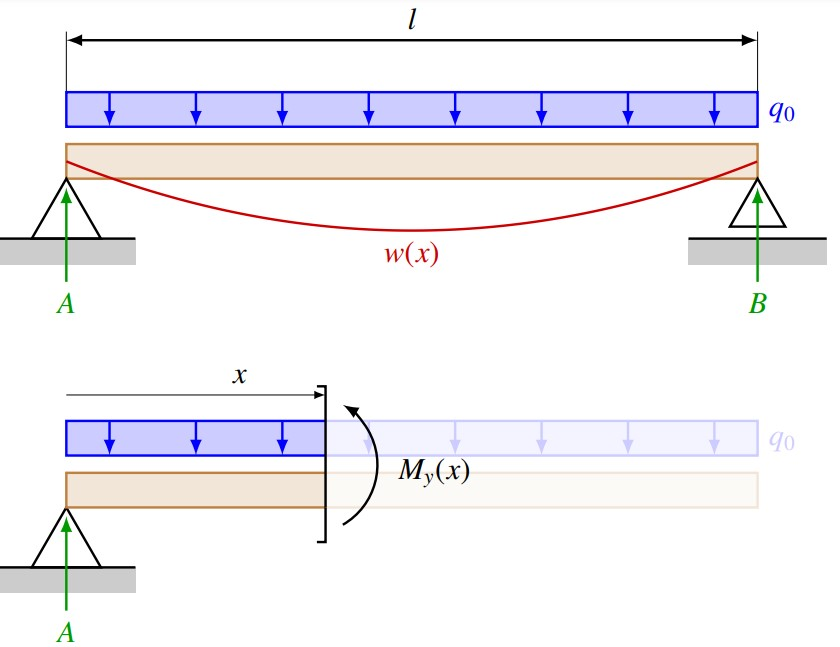
\includegraphics[width=0.8\textwidth]{papers/balken/images/teil2/HerleitungBaustatik.jpg}
\end{center}
\caption{Darstellung unsere Balke mit den Auflagern $A$ und $B$ und der Linienlast $q_0$.}
\end{figure}
gegeben ist:
\begin{equation}
	w''(x)=
	-\frac{M_y(x)}{EI_y}
	\rightarrow-M_y(x)=
	EI_y\cdot w''(x).
\end{equation}
Die Auflagerkräfte $A$ und $B$
\begin{equation}
	A=
	B=
	\frac{q_0\cdot L}{2}
\end{equation}
benötigen wir um die Schnittmomente an der Stelle $x$ zu berechnen:
\begin{equation}
	M_y(x)=
	A\cdot x-\frac{q_0\cdot x^2}{2}=
	\frac{q_0\cdot L}{2}\cdot x-\frac{q_0\cdot x^2}{2}.
\end{equation}
Moment ist gleich Kraft mal Hebelarm, daher setzen wir jetzt $My(x) = EIy \cdot w''(x)$ ein und erhalten
\begin{align}
		EI_y\cdot w''(x)&=
		\frac{q_0\cdot x^2}{2}-\frac{q_0\cdot L}{2}\cdot x
	\\
		EI_y\cdot w'\left(x\right)&=
		\frac{q_0}{2}\cdot\frac{1}{3}\cdot x^3-\frac{q_0\cdot 	L}{2}\cdot\frac{1}{2}\cdot x^2+C_1
	\\
		EI_y\cdot w\left(x\right)&=
		\frac{q_0}{6}\cdot\frac{1}{4}\cdot x^4-\frac{q_0\cdot 	L}{4}\cdot\frac{1}{3}\cdot x^3+C_1\cdot x+C_2
	\\
		EI_y\cdot w\left(x\right)&=
		\frac{q_0}{24}\cdot x^4-\frac{q_0\cdot L}{12}\cdot x^3+C_1\cdot x+C_2.
\end{align}

\subsection{Randbedingungen}
1. Randbedingung: Durchbiegung an der Stelle $x = 0$ ist 0. Wir setzen diese Wert in (13.73) ein und erhalten:
\begin{align}
		EI_y\cdot w\left(x\right)&=
		\frac{q_0}{24}\cdot x^4-\frac{q_0\cdot L}{12}\cdot x^3+C_1\cdot x+C_2
	\\
		0&=
		\frac{q_0}{24}\cdot0^4-\frac{q_0\cdot L}{12}\cdot0^3+C_1\cdot0+C_2
	\\
		C_2&=0.
\end{align}
2. Randbedingung: Durchbiegung an der Stelle $x = L$ ist auch 0.
\begin{align}
		EI_y\cdot w\left(x\right)&=
		\frac{q_0}{24}\cdot x^4-\frac{q_0\cdot L}{12}\cdot x^3+C_1\cdot x+C_2
	\\
		0&=
		\frac{q_0}{24}\cdot L^4-\frac{q_0\cdot L}{12}\cdot L^3+C_1\cdot L+0
	\\
		C_1&=
		\frac{q_0\cdot L^3}{24}.
\end{align}

\subsection{Gleichung der Biegelinie}
Daraus ergibt sich der Formel:
\begin{align}
		EI_y\cdot w\left(x\right)&=
		\frac{q_0}{24}\cdot x^4-\frac{q_0\cdot L}{12}\cdot x^3+\frac{q_0\cdot L^3}{24}\cdot x
	\\
		w&=
		\frac{1}{12EI_y}q_0\left(\frac{1}{2}x^4-Lx^3+\frac{1}{2}L^3x\right).
\end{align}
Das ist äquivalent zu dem, was wir bei der mathematischen Herleitung erhalten haben.

\subsection{Erläuterung der Annahmen und Randbedingungen}
Um die Berechnungen innerhalb der Balkentheorie pragmatischer zu gestalten, werden einige Vereinfachungen vorgenommen und die Randbedingungen festgelegt, unter denen sie gültig sind.
Dadurch können die Berechnungen vereinfacht und lösbar gemacht werden \cite{balken:Differentialgleichung-der-Biegelinie}.
Zu den Annahmen und Randbedingungen gehören folgende Aspekte:

\begin{enumerate}
	\item Die Balken werden als dünn angenommen, die hat zu bedeuten, dass die Dicke im Vergleich zur Länge des Balkens vernachlässigbar klein ist und deshalb für die Berechnung irrelevant ist.
	
	\item Die Balken sind eine konstante Linienlast ausgesetzt.
	
	\item Die Balken werden als ebene Struktur betrachtet, ohne signifikante Krümmungen und Verwindungen.
	
	\item Im unbelasteten Zustand bleiben Linienabschnitte, die senkrecht zur Mittelfläche stehen, auch im verformten Zustand gerade und senkrecht zur verformten Mittelfläche.
	
	\item Randbedingungen werden festgelegt, wobei die Art der Auflagerung oder Einspannung des Balkens berücksichtigt wird.
	Diese Randbedingungen sind in der untenstehenden Tabelle aufgeführt.
	
	\item Die Verformungen und Spannungen innerhalb des Balkens werden als vernachlässigbar klein betrachtet und können deshalb ausgeschlossen.
	
	\item Die Biegesteifigkeit des Balkens ist als konstant anzunehmen.
	
	\item Es wird angenommen, dass die Temperaturdifferenz, die zu Verformungen der Balkenachse führt, konstant ist, und daher ergibt seine zweite Ableitung Null.
	
	\item Die Belastungen des Balkens wirken senkrecht zur Achse.
\end{enumerate}
\begin{figure}
\begin{center}
	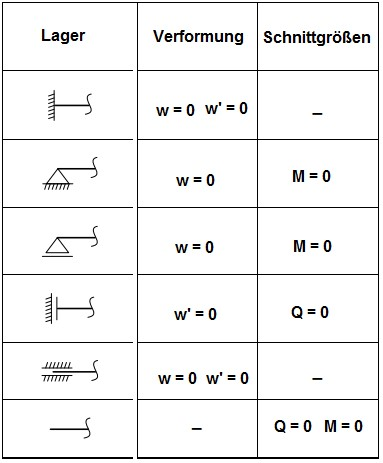
\includegraphics[width=0.4\textwidth]{papers/balken/images/teil2/Randbedingungen.jpg}
\end{center}
\caption{Tabelle der unterschiedlichen Randbedingungen für verschiedene Auflagertypen.}
\end{figure}
